% Graphic for TeX using PGF
% Title: D:\workspace\uos_pa_sph\doku\images\datenstruktur_eintraege.dia
% Creator: Dia v0.97.2
% CreationDate: Wed Sep 11 14:25:16 2013
% For: Nikki
% \usepackage{tikz}
% The following commands are not supported in PSTricks at present
% We define them conditionally, so when they are implemented,
% this pgf file will use them.
\ifx\du\undefined
  \newlength{\du}
\fi
\setlength{\du}{15\unitlength}
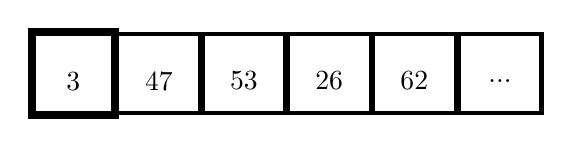
\begin{tikzpicture}
\pgftransformxscale{1.000000}
\pgftransformyscale{-1.000000}
\definecolor{dialinecolor}{rgb}{0.000000, 0.000000, 0.000000}
\pgfsetstrokecolor{dialinecolor}
\definecolor{dialinecolor}{rgb}{1.000000, 1.000000, 1.000000}
\pgfsetfillcolor{dialinecolor}
\definecolor{dialinecolor}{rgb}{1.000000, 1.000000, 1.000000}
\pgfsetfillcolor{dialinecolor}
\fill (46.050000\du,22.150000\du)--(46.050000\du,24.150000\du)--(48.050000\du,24.150000\du)--(48.050000\du,22.150000\du)--cycle;
\pgfsetlinewidth{0.200000\du}
\pgfsetdash{}{0pt}
\pgfsetdash{}{0pt}
\pgfsetmiterjoin
\definecolor{dialinecolor}{rgb}{0.000000, 0.000000, 0.000000}
\pgfsetstrokecolor{dialinecolor}
\draw (46.050000\du,22.150000\du)--(46.050000\du,24.150000\du)--(48.050000\du,24.150000\du)--(48.050000\du,22.150000\du)--cycle;
% setfont left to latex
\definecolor{dialinecolor}{rgb}{0.000000, 0.000000, 0.000000}
\pgfsetstrokecolor{dialinecolor}
\node at (47.050000\du,23.337500\du){3};
\definecolor{dialinecolor}{rgb}{1.000000, 1.000000, 1.000000}
\pgfsetfillcolor{dialinecolor}
\fill (48.110000\du,22.200000\du)--(48.110000\du,24.100000\du)--(50.110000\du,24.100000\du)--(50.110000\du,22.200000\du)--cycle;
\pgfsetlinewidth{0.100000\du}
\pgfsetdash{}{0pt}
\pgfsetdash{}{0pt}
\pgfsetmiterjoin
\definecolor{dialinecolor}{rgb}{0.000000, 0.000000, 0.000000}
\pgfsetstrokecolor{dialinecolor}
\draw (48.110000\du,22.200000\du)--(48.110000\du,24.100000\du)--(50.110000\du,24.100000\du)--(50.110000\du,22.200000\du)--cycle;
% setfont left to latex
\definecolor{dialinecolor}{rgb}{0.000000, 0.000000, 0.000000}
\pgfsetstrokecolor{dialinecolor}
\node at (49.110000\du,23.337500\du){47};
\definecolor{dialinecolor}{rgb}{1.000000, 1.000000, 1.000000}
\pgfsetfillcolor{dialinecolor}
\fill (50.161077\du,22.198863\du)--(50.161077\du,24.098863\du)--(52.161077\du,24.098863\du)--(52.161077\du,22.198863\du)--cycle;
\pgfsetlinewidth{0.100000\du}
\pgfsetdash{}{0pt}
\pgfsetdash{}{0pt}
\pgfsetmiterjoin
\definecolor{dialinecolor}{rgb}{0.000000, 0.000000, 0.000000}
\pgfsetstrokecolor{dialinecolor}
\draw (50.161077\du,22.198863\du)--(50.161077\du,24.098863\du)--(52.161077\du,24.098863\du)--(52.161077\du,22.198863\du)--cycle;
% setfont left to latex
\definecolor{dialinecolor}{rgb}{0.000000, 0.000000, 0.000000}
\pgfsetstrokecolor{dialinecolor}
\node at (51.161077\du,23.336363\du){53};
\definecolor{dialinecolor}{rgb}{1.000000, 1.000000, 1.000000}
\pgfsetfillcolor{dialinecolor}
\fill (52.212855\du,22.198863\du)--(52.212855\du,24.098863\du)--(54.212855\du,24.098863\du)--(54.212855\du,22.198863\du)--cycle;
\pgfsetlinewidth{0.100000\du}
\pgfsetdash{}{0pt}
\pgfsetdash{}{0pt}
\pgfsetmiterjoin
\definecolor{dialinecolor}{rgb}{0.000000, 0.000000, 0.000000}
\pgfsetstrokecolor{dialinecolor}
\draw (52.212855\du,22.198863\du)--(52.212855\du,24.098863\du)--(54.212855\du,24.098863\du)--(54.212855\du,22.198863\du)--cycle;
% setfont left to latex
\definecolor{dialinecolor}{rgb}{0.000000, 0.000000, 0.000000}
\pgfsetstrokecolor{dialinecolor}
\node at (53.212855\du,23.336363\du){26};
\definecolor{dialinecolor}{rgb}{1.000000, 1.000000, 1.000000}
\pgfsetfillcolor{dialinecolor}
\fill (54.264633\du,22.198863\du)--(54.264633\du,24.098863\du)--(56.264633\du,24.098863\du)--(56.264633\du,22.198863\du)--cycle;
\pgfsetlinewidth{0.100000\du}
\pgfsetdash{}{0pt}
\pgfsetdash{}{0pt}
\pgfsetmiterjoin
\definecolor{dialinecolor}{rgb}{0.000000, 0.000000, 0.000000}
\pgfsetstrokecolor{dialinecolor}
\draw (54.264633\du,22.198863\du)--(54.264633\du,24.098863\du)--(56.264633\du,24.098863\du)--(56.264633\du,22.198863\du)--cycle;
% setfont left to latex
\definecolor{dialinecolor}{rgb}{0.000000, 0.000000, 0.000000}
\pgfsetstrokecolor{dialinecolor}
\node at (55.264633\du,23.336363\du){62};
\definecolor{dialinecolor}{rgb}{1.000000, 1.000000, 1.000000}
\pgfsetfillcolor{dialinecolor}
\fill (56.326923\du,22.198863\du)--(56.326923\du,24.098863\du)--(58.326923\du,24.098863\du)--(58.326923\du,22.198863\du)--cycle;
\pgfsetlinewidth{0.100000\du}
\pgfsetdash{}{0pt}
\pgfsetdash{}{0pt}
\pgfsetmiterjoin
\definecolor{dialinecolor}{rgb}{0.000000, 0.000000, 0.000000}
\pgfsetstrokecolor{dialinecolor}
\draw (56.326923\du,22.198863\du)--(56.326923\du,24.098863\du)--(58.326923\du,24.098863\du)--(58.326923\du,22.198863\du)--cycle;
% setfont left to latex
\definecolor{dialinecolor}{rgb}{0.000000, 0.000000, 0.000000}
\pgfsetstrokecolor{dialinecolor}
\node at (57.326923\du,23.336363\du){...};
\end{tikzpicture}
